\chapter{Research Internship, Presentations and Service Work}

\section{Internship at CERN}

Important  advances in this thesis project were accomplished during the one-year internship at CERN, working in collaboration with the B2G physics analysis group. This internship occurred between July 2014 and June 2015, and the commissioning of the analysis framework and several optimizations were performed during this period.

\begin{figure}[htb]
\begin{center}
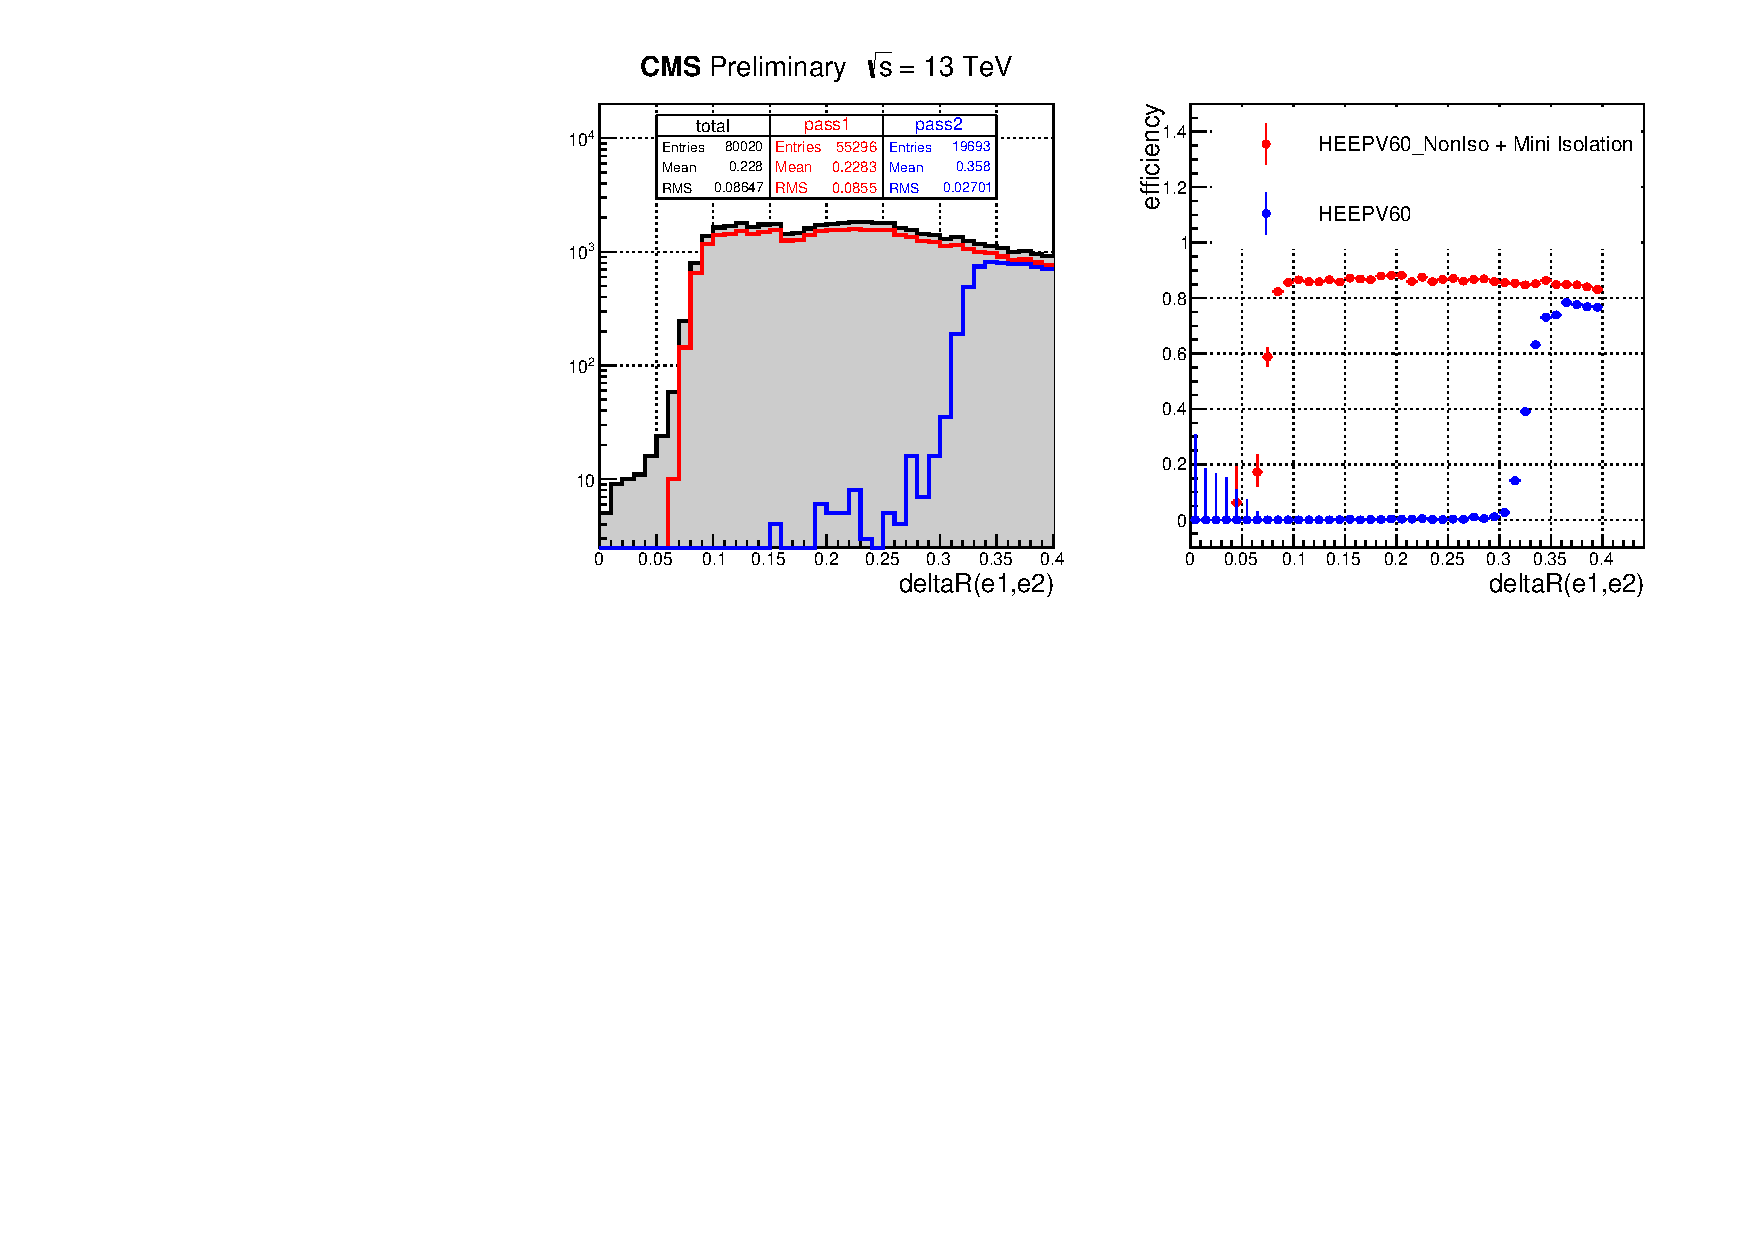
\includegraphics[scale=0.8]{figures/systematics/deltaRleplep_heep.pdf}
\caption[Electron efficiency as function of deltaR]{Electron efficiency as function of $\Delta R$.}
\label{boostedDR}
\end{center}
\end{figure}

Another activity during the stay at CERN involved the studies on electron identification and isolation. In hadron colliders like the LHC, a proper isolation of electrons from the hadronic contamination is important to achieve high levels of efficiency and improve the sensitivity of the searches. The isolation of a pair of boosted electrons is particularly difficult because the presence of one electron may spoil the isolation of the other. 

This behavior was studied in Monte Carlo simulations, as shown in Fig.~\ref{boostedDR}. In this context, there were proposals to apply a new technique called mini-isolation characterized with a variable isolation cone. In the beginning the mini-isolation seemed to be an acceptable solution for the problem of the isolation of boosted electrons, but there were complications regarding the performance of the technique in real data. At the end, the mini-isolation technique was not adopted, and the analysis opted for the standard particle-flow based isolation suggested by the electron physics object group.

The list of presentations given at the diboson resonance meeting, which is internal for members of the CMS Collaboration, are shown in Table \ref{meetings}.  

\vspace{0.5cm}
\begin{table}[htb]
\centering
\caption{Presentations at CMS internal meeting.}
\label{meetings}
\begin{tabular}{cc} \hline
&\\[-0.2cm]
{\bf Date} & {\bf Link to the Agenda} \\[0.2cm]
\hline\hline
%{\footnotesize 24 Nov 2016} & \href{https://indico.cern.ch/event/590809/}{\footnotesize https://indico.cern.ch/event/580809/} \\
13 Aug 2014 & \href{https://indico.cern.ch/event/334733}{https://indico.cern.ch/event/334733} \\     
04 Nov 2014 &  \href{https://indico.cern.ch/event/348912}{https://indico.cern.ch/event/348912} \ \\
14 Nov 2014 & \href{https://indico.cern.ch/event/338802}{https://indico.cern.ch/event/338802} \ \\
26 Nov 2014 &  \href{https://indico.cern.ch/event/349870}{https://indico.cern.ch/event/349870} \ \\
01 Dec 2014 & \href{https://indico.cern.ch/event/355405}{https://indico.cern.ch/event/355405} \ \\
10 Dec 2014 &  \href{https://indico.cern.ch/event/357685}{https://indico.cern.ch/event/357685} \ \\
21 Jan 2015 &  \href{https://indico.cern.ch/event/367603}{https://indico.cern.ch/event/367603} \ \\
28 Jan 2015 &  \href{https://indico.cern.ch/event/369935}{https://indico.cern.ch/event/369935} \ \\
02 Feb 2015 & \href{https://indico.cern.ch/event/369661}{https://indico.cern.ch/event/369661} \ \\
25 Mar 2015 & \href{https://indico.cern.ch/event/383553}{https://indico.cern.ch/event/383553} \ \\
01 Apr 2015 & \href{https://indico.cern.ch/event/384925}{https://indico.cern.ch/event/384925} \\\
13 Apr 2015 & \href{https://indico.cern.ch/event/387620}{https://indico.cern.ch/event/387620} \ \\
13 May 2015 & \href{https://indico.cern.ch/event/394192}{https://indico.cern.ch/event/394192} \ \\
20 May 2015 & \href{https://indico.cern.ch/event/395573}{https://indico.cern.ch/event/395573} \ \\
27 May 2015 & \href{https://indico.cern.ch/event/396649}{https://indico.cern.ch/event/396649} \ \\
01 Jul 2015 & \href{https://indico.cern.ch/event/405140}{https://indico.cern.ch/event/405140} \ \\
06 Jul 2015 & \href{https://indico.cern.ch/event/405333}{https://indico.cern.ch/event/405333} \ \\
15 Jul 2015 & \href{https://indico.cern.ch/event/433384}{https://indico.cern.ch/event/433384} \ \\
\hline
\end{tabular}
\end{table}


\section{Service Work to the Collaboration}
In addition to the research activities, every collaborator in CMS is appointed to a service work in order to guarantee the good operation of the experiment. In this section we describe the specific duties that were performed in 2016. 

The CMS trigger system is responsible for selecting in real-time those interesting events that should be recorded for offline analysis. Every release of the CMS software (CMSSW) is accompanied with a set of validation samples with the end of monitoring the performance of individual triggers. The responsibilities of the trigger validator include:

\begin{compact_itemize}
\item Make systematic comparisons between consecutive CMSSW releases.
\item Maintain the validation packages for Susy and Exotica analysis groups.
\item Report to the trigger studies group in charge of the strategy for trigger evolution and monitoring.
\end{compact_itemize}

\begin{figure}[htb]
\begin{center}
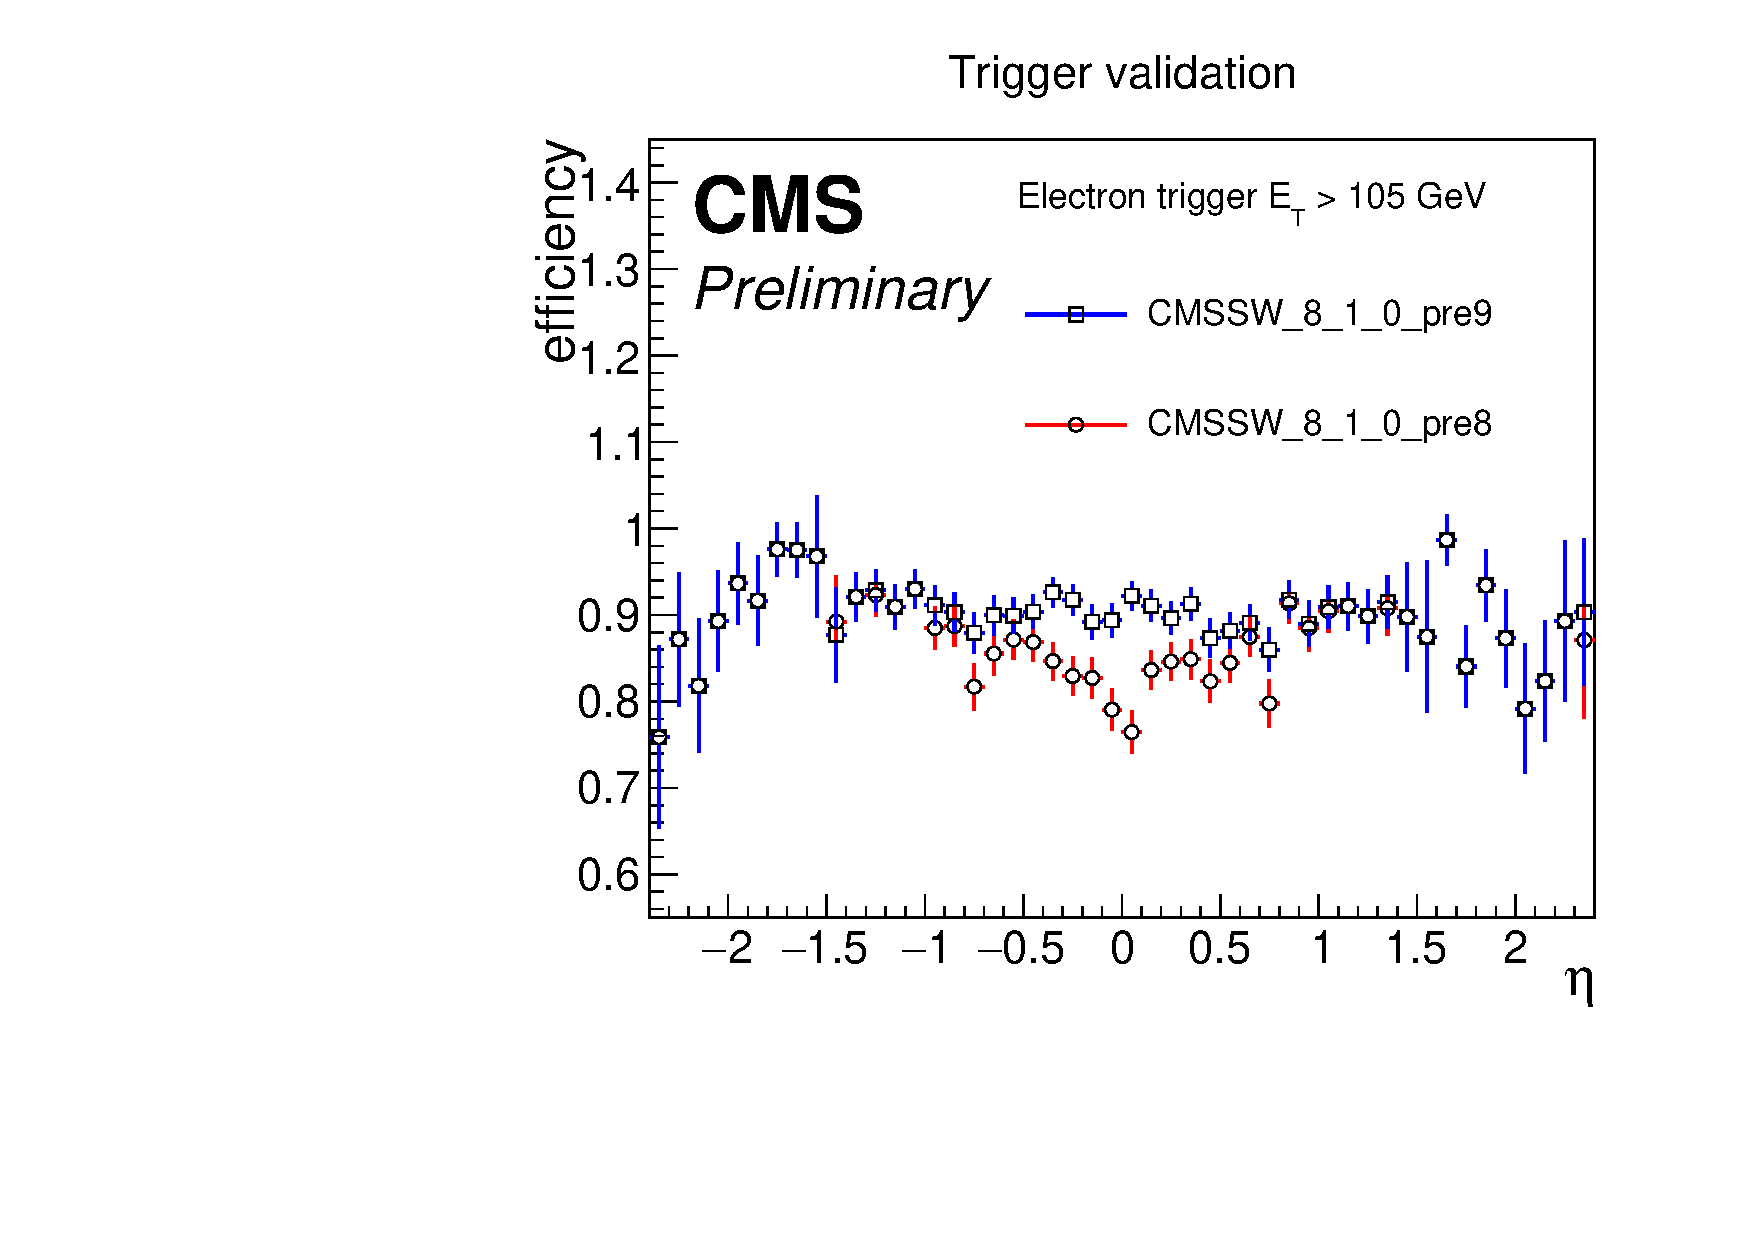
\includegraphics[scale=0.55]{figures/fits/triggerValidation.pdf}
\caption{Efficiency of the high energy electron trigger $E_{\rm T}> 105$ GeV as function of pseudorapidity $\eta$. The comparison of two consecutive pre-releases of the CMSSW is important to reveal either an expected change in the configuration of the trigger or the diagnostic of systematic problems.}
\label{monitor}
\end{center}
\end{figure}


Figure \ref{monitor} shows one of the monitor elements for trigger validation with the efficiency to select high energy electrons ($E_{\rm T}> 105$ GeV). In this particular example we observe discrepancies in the efficiency in the central region of $\eta$, which is an indication of either an expected change in the configuration of the trigger or an actual issue. The validations between consecutive releases of the CMSSW is important to spot as early as possible any problem that can affect the normal behaviour of the trigger. Since the CMSSW is continuously evolving, the validation has to be performed in a regular weekly basis. 


\begin{table}[htb]
\centering
\caption[Trigger validation campaigns in 2016]{Trigger validation campaigns in 2016.}
\label{validations}
\begin{tabular}{lc} \hline
&\\[-0.2cm]
{\bf Release Name} & {\bf Date}  \\[0.2cm]
\hline\hline
{ 8\_1\_0\_PRE4}           & { May 15} \\
{ 8\_1\_0\_PRE5}           & { May 29} \\
{ 8\_1\_0\_PRE6}           & { Jun 15} \\
{ 8\_0\_10\_HLT}           & { Jun 16} \\
{ 8\_1\_0\_PRE8}           & { Jul 15} \\
{ 8\_1\_0\_PRE9}           & { Jul 29} \\
{ 8\_0\_16}                & { Aug 13} \\
{ 8\_0\_16\_Tranch4GT}     & { Aug 22} \\
{ 8\_1\_0\_PRE10}          & { Sep 1 } \\
{ 8\_0\_19\_Tranch4GT}     & { Sep 13} \\
{ 8\_1\_0\_PRE11}          & { Sep 22} \\
{ 8\_1\_0\_PRE12}          & { Oct 11} \\
{ 8\_1\_0\_PRE15}          & { Nov 04} \\
{ 8\_1\_0\_PRE16}          & { Nov 22} \\
\hline
\end{tabular}
\end{table}

\section{National and International Presentations}

In addition to the CMS internal presentations, the results derived from this project were presented in public conferences for a wider audience. 

\begin{itemize}
\item {\bf November 2014}: Oral presentation at ``CMS Exotica Workshop 2014", Madrid (Spain).
\item {\bf September 2015}: Oral presentation at ``XXXVI Encontro Nacional de F\'isica de Part\'iculas e Campos", Caxambu, MG (Brazil) \cite{ENF2015}.
\item {\bf November 2015}: Oral presentation at II Simp\'osio de F\'isica, Astronomia e Meteorologia, Bauru, SP (Brazil).
\item {\bf May 2016}: Pre-approval presentation of the analysis to the B2G conveners.
\item {\bf July 2016}: Approval of the analysis by the CMS Collaboration \cite{CMS-PAS-B2G-16-010}.
\item {\bf August 2016}: Poster ``Search for new resonances in the merged jet + dilepton final state in CMS''
presented on behalf of the CMS collaboration at the 38th International Conference on High Energy Physics (ICHEP 2016) \cite{Proceedings:2016pwg}, Chicago (USA) --- \href{https://pos.sissa.it/archive/conferences/282/757/ICHEP2016_757.pdf}{Proceedings of Science}.
\item {\bf September 2016}: Oral presentation at "Encontro de F\'isica 2016'' (ENF 2016) \cite{ENF2016}, Natal, RN (Brazil).
\end{itemize}  



%\section{Future Perspectives}
